\documentclass{beamer}


\usepackage{multicol,lipsum,caption}
\usepackage{amsmath,booktabs,verbatim,tikz} \usetikzlibrary{shapes.geometric, arrows,positioning,matrix,calc}
%\usepackage{mathptmx}

\usetheme[progressbar=frametitle]{metropolis}
\setbeamertemplate{frame numbering}[fraction]
\useoutertheme{metropolis}
\useinnertheme{metropolis}
\usefonttheme{metropolis}
\usecolortheme{spruce}
\setbeamercolor{background canvas}{bg=white}

\title{Neural Network, Genetic Algorithm and Composite Material}
\author{Huiyao Zhang}
\institute{Kyoto Institue of Technology}
\date{05-25-2020}
\setbeamertemplate{itemize/enumerate body begin}{\large}

\begin{document}
\begin{frame}
    \titlepage
\end{frame}




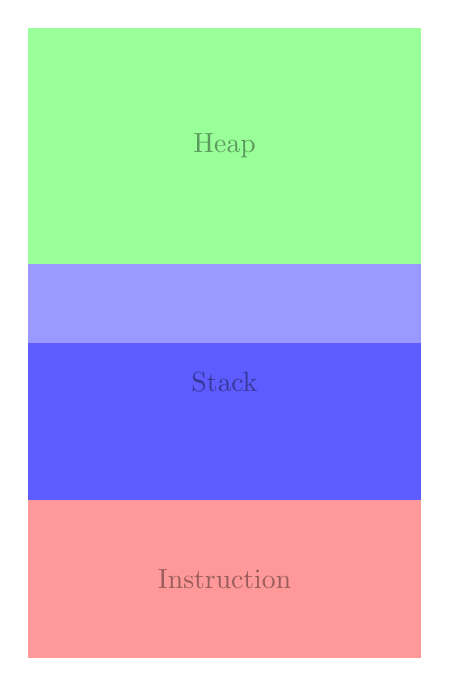
\begin{tikzpicture}[opacity=0.4]
    \fill[red] (0,0) rectangle  (5,2);
    \fill[blue] (0,2) rectangle (5,5);
    \fill[blue] (0,2) rectangle (5,3);
    \fill[blue] (0,3) rectangle (5,4);
    \fill[green] (0,5) rectangle (5,8);

    \node at (2.5,1) {Instruction};
    \node at (2.5,3.5) {Stack};
    \node at (2.5,6.5) {Heap};

\end{tikzpicture}

\begin{frame}[c]{Content} 
    \begin{enumerate}
        \item Genetic Algorithm for Multimodal Problem(Solved)
        \item Neural Network Design(Solved)
        \item Composite Material(Unsolved)
    \end{enumerate}
\end{frame}

\begin{frame}{Genetic Algorithm}
\begin{columns}[c]
    \begin{column}{0.6\textwidth}
   
        \begin{equation}
        s h\left(d_{i, j}\right)=\left\{\begin{array}{ll}{1-\left(\frac{d_{i, j}}{\sigma_{s h}}\right)^{\alpha_{s h}}} 
            & {\text { if } d_{i, j}<\sigma_{s h}} \\ 
        {0} & {\text { otherwise }}\end{array}\right.
        \end{equation}
        where $d_{i,j}$ denotes distance between two individuals, $\alpha_{s h}$
        is a constant number and $\sigma_{s h}$ is the radius of niches.
    \end{column}
    \begin{column}{0.4\textwidth}
        \begin{center}
        \captionof{table}{GA Parameters}
        \begin{tabular}{cc}
            \toprule
            parameter & value \\
            \midrule
            generation           & 50 \\
            length      & 16 \\
            encoding& binary encoding\\
            cross& one-point \\
            mutation& none \\
            \bottomrule
        \end{tabular}
        \label{tab:GA}
        \end{center}
    \end{column}
\end{columns}



\end{frame}

\begin{frame}{Genetic Algorithm}
    \begin{columns}[c]
    \begin{column}{0.5\textwidth}
        Target Function
        \begin{equation}
        f_{1}(x)=\sin^{6}(5.1 \pi x+0.5)
        \end{equation}
    \end{column}
    \begin{column}{0.5\textwidth}
        \begin{center}
              \includegraphics[width=0.8\linewidth]{GA_images/example-sin.png}
              \captionof{figure}{Target Function}
        \end{center}
        \begin{center}
              \includegraphics[width=0.8\linewidth]{GA_images/example-sin-result.png}
              \captionof{figure}{Result}
        \end{center}
    \end{column}

\end{columns}


\end{frame}

\begin{frame}{Genetic Algorithm}
    \begin{columns}[c]
    \begin{column}{0.5\textwidth}
        Target Function
        \begin{equation}
        \mathrm{f}_{2}(\mathrm{x})=\mathrm{f}_{1}(\mathrm{x}) \cdot
        \mathrm{e}^{\left[-4 \ln 2
        \frac{(\mathrm{x}-0.086)^{2}}{0.8^{2}}\right]}
        \end{equation}
    \end{column}
    \begin{column}{0.5\textwidth}
        \begin{center}
              \includegraphics[width=0.8\linewidth]{GA_images/example-composite-sin.png}
              \captionof{figure}{Target Function}
        \end{center}
        \begin{center}
      \includegraphics[width=\linewidth]{GA_images/example-composite-sin-result.png}
              \captionof{figure}{Result}
        \end{center}
    \end{column}
\end{columns}
\end{frame}



\begin{frame}{Neural Network Design}
    \begin{columns}
    \begin{column}{0.7\textwidth}

        \begin{center}
            \includegraphics[width=1.0\linewidth]{GA_images/neural-network-design.png}
              \captionof{figure}{Bit String Genotype}
        \end{center}
    \end{column}
    \begin{column}{0.4\textwidth}
        \begin{center}
              \includegraphics[width=0.8\linewidth]{GA_images/ga-neural-network.png}
              \captionof{figure}{Architecture}
        \end{center}
    \end{column}
\end{columns}
\end{frame}


\begin{frame}{Neural Network Design}
    \begin{columns}
    \begin{column}{0.5\textwidth}
        \begin{center}
              \includegraphics[width=0.8\linewidth]{GA_images/adaboost.png}
              \captionof{figure}{Adaboost}
        \end{center}
        \begin{center}
              \includegraphics[width=0.8\linewidth]{GA_images/neural-network-train.png}
              \captionof{figure}{Train Process of Neural Network with Toy Data }
        \end{center}
    \end{column}
    \begin{column}{0.5\textwidth}
        \begin{center}
              \includegraphics[width=0.8\linewidth]{GA_images/neural-network.png}
              \captionof{figure}{Topology of Neural Network}
        \end{center}
    \end{column}
\end{columns}
\end{frame}



\begin{frame}{Composite Material}
    \begin{columns}[c]
    \begin{column}{0.5\textwidth}
        \begin{itemize}
            \item  How to get these three things work together ?
        \end{itemize}
    \end{column}
    \begin{column}{0.5\textwidth}
        \begin{center}
              \includegraphics[width=0.8\linewidth]{GA_images/composite-material.png}
              \captionof{figure}{Composite Material}
        \end{center}
    \end{column}
\end{columns}
\end{frame}
\end{document}
